\chapter{State of the art}
\label{chap:sota}

\section{Object detection}

Object detection is one of the most fundamental and challenging problems in computer vision \cite{zou2019object}. This task can be defined as follows: given an image, determine whether or not there are instances of a predefined set of objects, usually referred as classes, and, if present, return the location of each instance \cite{liu2020deep}. The spatial location of an object in an image can be represented using bounding boxes.

Object detection has initially been addressed using handcrafted features and shallow trainable architectures.
With the rapid development in deep learning, more powerful techniques are used to address the problems existing in traditional architectures \cite{zhao2019object}. 

As described in \cite{zhao2019object}, the frameworks of object detection methods can mainly be categorized into two types:
\begin{enumerate}
    \item Generating region proposals at first and then classifying each proposal into different object categories.
    \item Adopting a unified framework to achieve final results (categories and locations) directly.
\end{enumerate} 

\subsection{YOLO}
YOLO (you only look once) \cite{redmon2016you} is a model for object detection composed of a single neural network which treats object detection as a regression problem: given an image as input it produces bounding box coordinates and associated class probabilities. Since the predictions are performed directly on the input image without requiring complex pipelines, YOLO is very efficient and can lead to real-time object detection.

\begin{figure}
    \begin{center}
        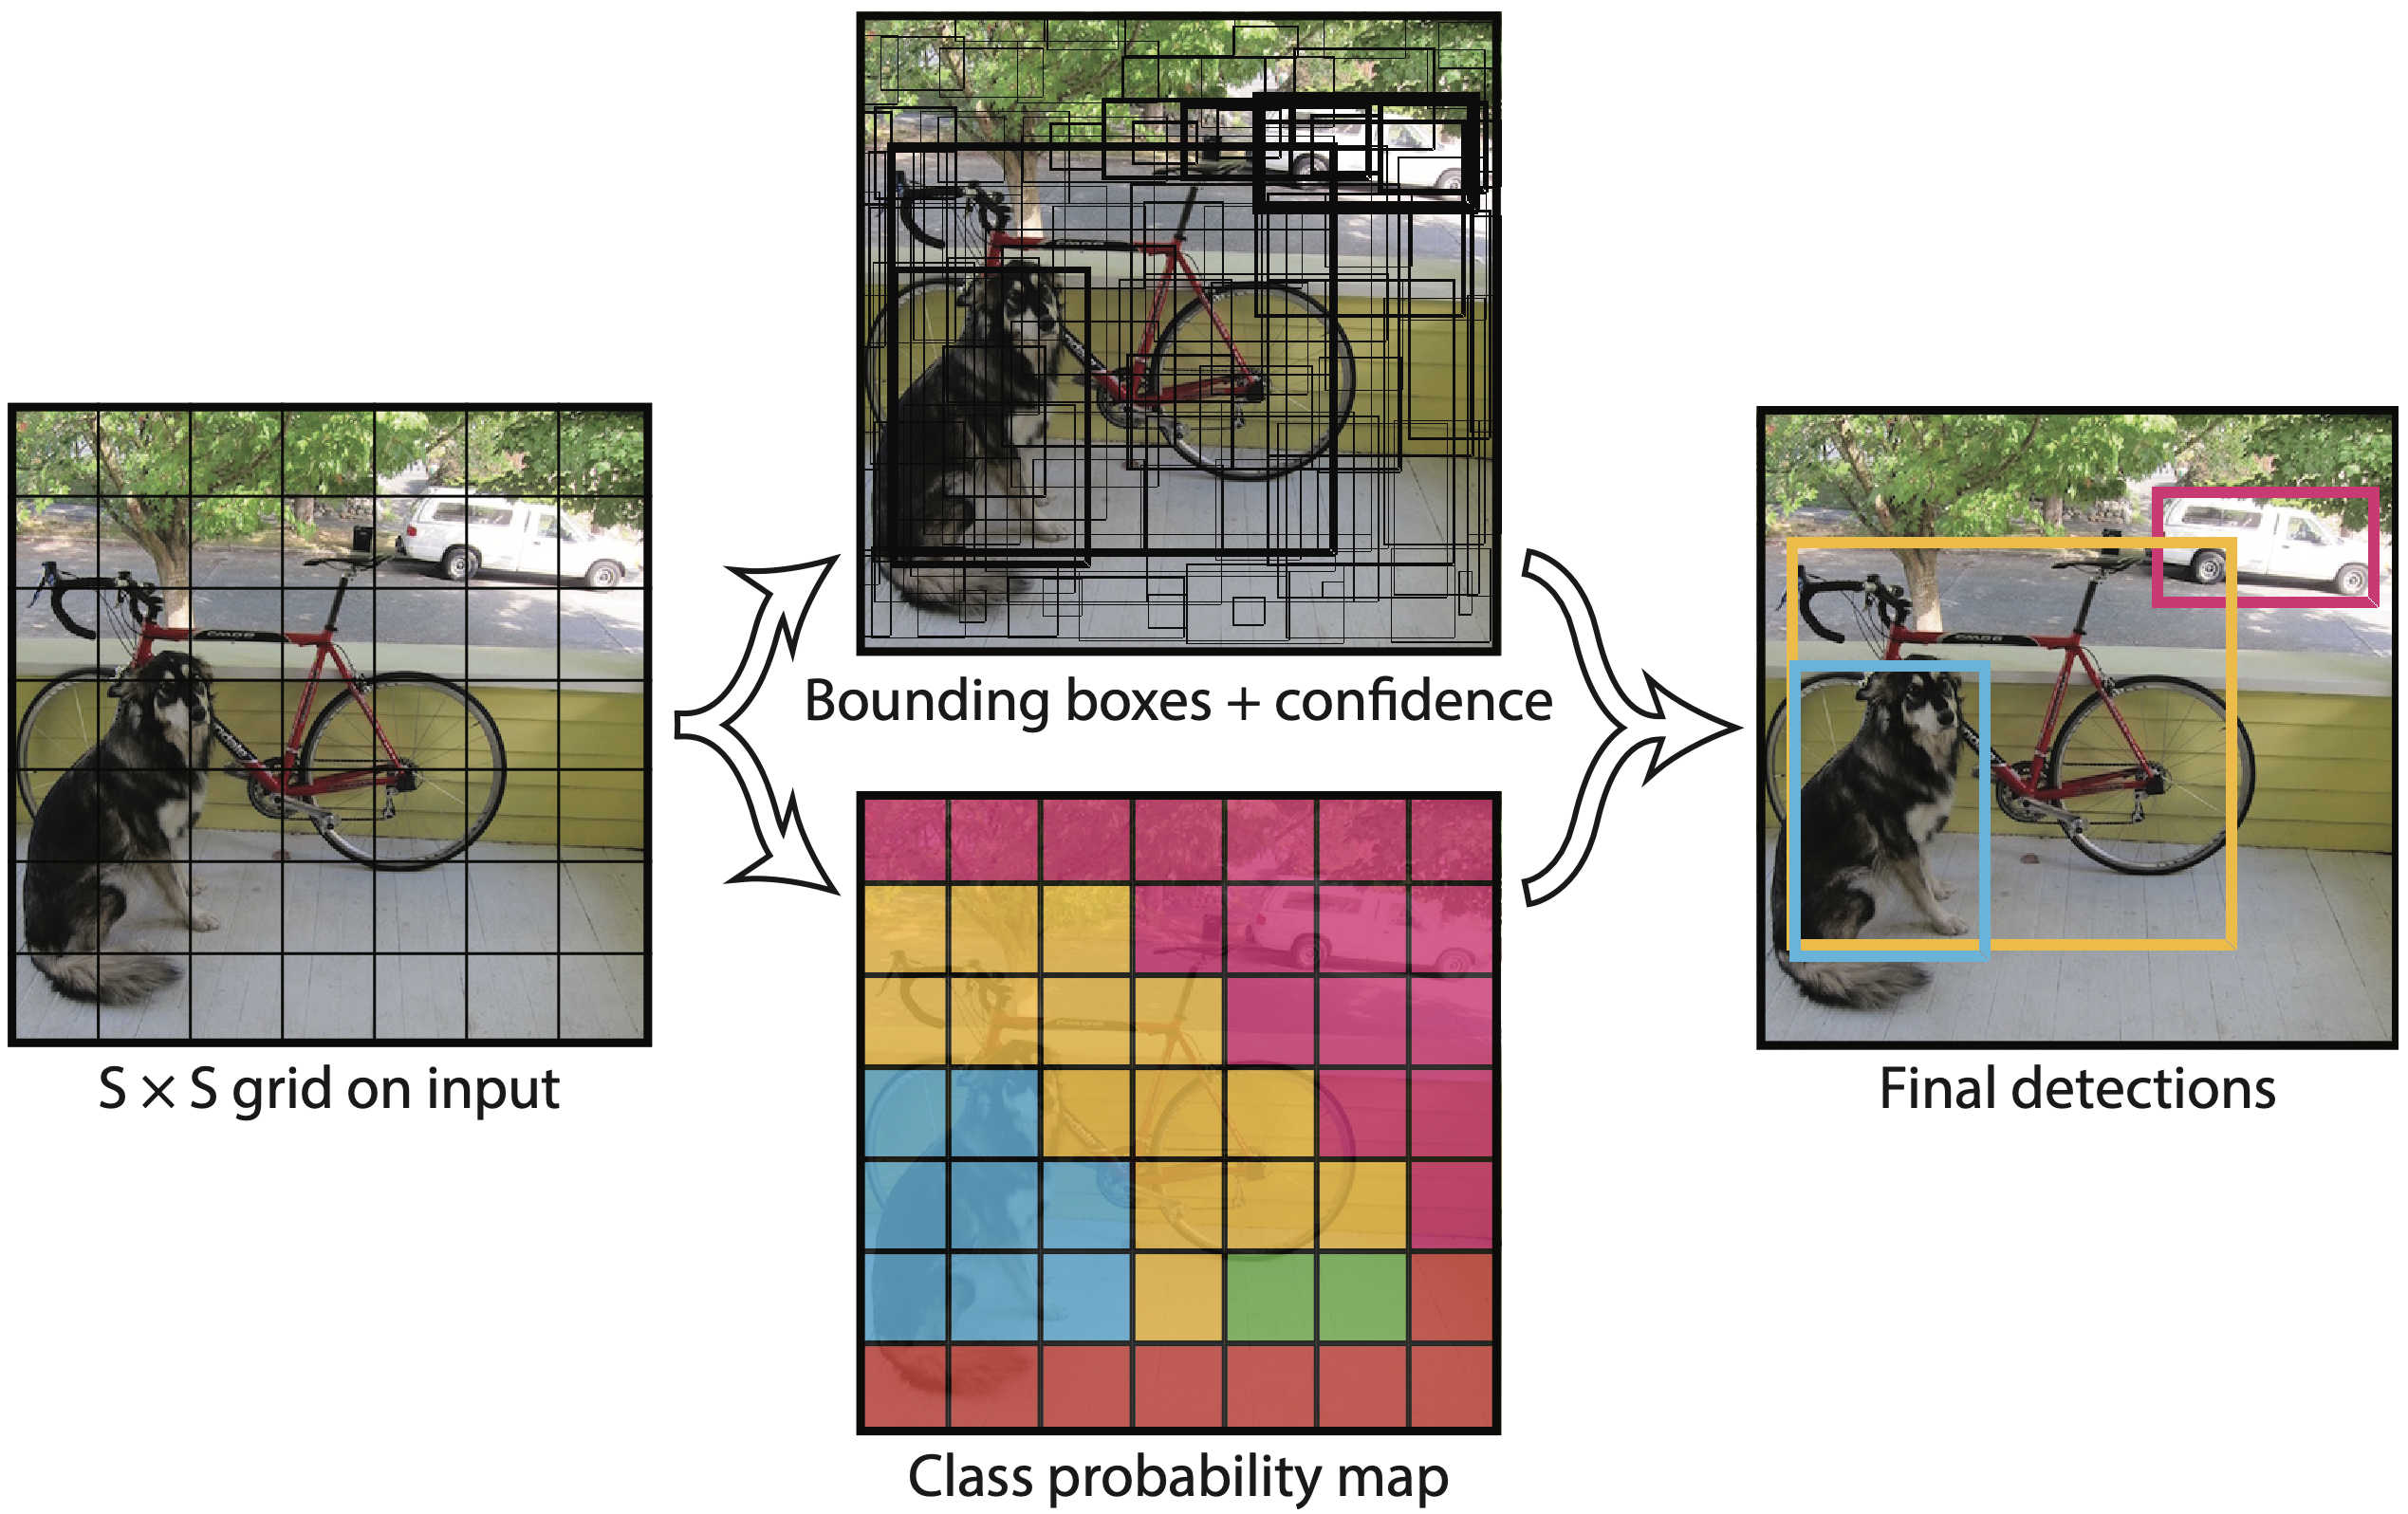
\includegraphics[width=\columnwidth]{images/yolo-model.png}
    \end{center}
    \caption{Pipeline of YOLO \cite{redmon2016you}.}
    \label{fig:yolo-model}
\end{figure}

In YOLO, the input image is divided into a $S \times S$ grid and the cell in which the center of the object falls is responsible for the detection of that object.
A grid cell can predict more than one bounding box, where each prediction consists of an array composed by 5 elements: center of the bounding identified by the coordinates $x$ and $y$, dimensions of the box $w$ and $h$, and the confidence score of that bounding box representing an object. At the same time, regardless of the number of boxes in each cell, C conditional probabilities $\Pr(Class_i | Object)$ are computed in each grid cell. The final prediction will be encoded as an $S \times S \times (B * 5 + C)$ tensor. The model pipeline is shown in \autoref{fig:yolo-model}

The model is trained via the optimization of the following loss function:

\begin{equation}\label{eq:yolo-loss}
    \begin{split}
        \mathcal{L} \quad =  \quad  &
            \lambda_{coord} \sum_{i=0}^{S^2} \sum_{j=0}^{B} \mathbb{1}_{ij}^{obj}
            [(x_i - \hat x_i)^2 + (y_i - \hat y_i)^2]\\
            \quad + \quad & \lambda_{coord} \sum_{i=0}^{S^2} \sum_{j=0}^{B} \mathbb{1}_{ij}^{obj}
                [(\sqrt{w_i} - \sqrt{\hat w_i})^2 + (\sqrt{h_i} - \sqrt{\hat h_i})^2]\\
            \quad + \quad & \sum_{i=0}^{S^2} \sum_{j=0}^{B} \mathbb{1}_{ij}^{obj}
                (C_i - \hat C_i)^2 \; + \; \lambda_{noobj} \sum_{i=0}^{S^2} \sum_{j=0}^{B} \mathbb{1}_{ij}^{noobj}(C_i - \hat C_i)^2\\
            \quad + \quad & \sum_{i=0}^{S^2} \mathbb{1}_{i}^{obj} \sum_{c \in classes}
                (p_i(c) - \hat p_i (c))^2\\
    \end{split}
\end{equation}
where,
\begin{align*}
    \mathbb{1}_{ij}&=\left\{
        \begin{array}{@{}ll@{}}
            1, & \text{if the } j \text{-th bbox in cell } i \text{ is responsible fot that prediction}\\
            0, & \text{otherwise}
        \end{array}\right.\\
    \mathbb{1}_{i}&=\left\{
        \begin{array}{@{}ll@{}}
            1, & \text{if there is an object in cell}\ i \\
            0, & \text{otherwise}
        \end{array}\right.
\end{align*}


The loss function in \autoref{eq:yolo-loss} considers both detection and classification. A bounding box can be defined by its center in addition to the height and width. The first row of the loss function is responsible for minimizing the difference between the predicted center and the ground truth, and the second row minimize the difference between width and height.
The third row penalizes the neural network if it predicts an object whereas it is not present and vice versa. The last row of the loss function is the mean squared error between the real class and the predicted one, hence it is responsible to match the real class.


Over the years, several versions of YOLO have came up, starting from the first up to fifth version \cite{redmon2016you, redmon2017yolo9000, redmon2018yolov3, bochkovskiy2020yolov4, glenn_jocher_2021_5563715}. YOLOv5 represents the state of the art for object detection, and compared with the most recent models it is among the best performing ones \cite{zaidi2022survey}.

\section{Logo recognition}
\label{sec:sota-logoyolo}

A general pipeline for logo detection and recognition consists in logo region proposal followed by a classifier specifically trained for logo classification, as proposed by Bianco et al. in \cite{bianco2017deep} or by Fehérvári et al. in \cite{fehervari2019scalable}.

Another approach presented by Wang et al. \cite{wang2022logodet} involves a model based on YOLOv3 \cite{redmon2018yolov3} used to produce both bounding boxes and classification for each detected logo. The proposed model is called Logo-YOLO, which is essentially the same version of YOLOv3 with some changes to the loss function described in \autoref{eq:yolo-loss} and the re-computation of the anchors sizes. The modified loss function utilizes the Focal Loss \cite{lin2017focal} to solve the problem of the logos which are small objects to the background, and the  CIoU loss \cite{zheng2020distance} to obtain more accurate and faster regression of the bounding boxes.

The issue with this approaches is the closed-world assumption which does not apply in the case of logo recognition, as discussed in \autoref{sec:logodet-intro}. This is the purpose behind works such as \cite{fehervari2019scalable}. The authors of the paper propose a method based on Distance Metric Learning (DML) using deep learning techniques called SoftTriple Loss presented in \cite{qian2019softtriple}. This work aims to achieve logo recognition via metric learning, where a model learns the similarity of different objects in a latent space, thus being able to deal with a large number of previously unseen classes exploiting the distances of objects in the latent space.

Another work based on DML has been presented by Li et al. \cite{li2022seetek} and can be considered as an extension to \cite{fehervari2019scalable}. In this work the authors enrich the latent space learned by DML with text features contained in the logos. The authors highlight how a large number of logos have remarkable amount of text or (stylized) letters, for this reason, in addition to visual features, they consider text features as relevant information for logo classification.

\section{Class incremental learning}
Traditional supervised learning systems are trained in closed-world for a fixed
number of classes, that requires all the training data to be available before training.
The problem of Class Incremental Learning (CIL) aims to design algorithms that can learn new concepts in a sequential way and eventually perform well on all observed classes \cite{yan2021dynamically}.

To extend a trained model on new classes, a large amount of labeled data for both new
and old classes is necessary for network finetuning. Otherwise, if the dataset of old classes is no
longer available, finetuning a deployed model with
new classes can lead to the catastrophic forgetting
problem \cite{serra2018overcoming, zhang2021few, mccloskey1989catastrophic}. Catastrophic forgetting means that a Deep Neural Network (DNN) degrades performance on old classes when retrained on new ones.

\subsection{Problem setup}


\begin{figure}
    \begin{center}
        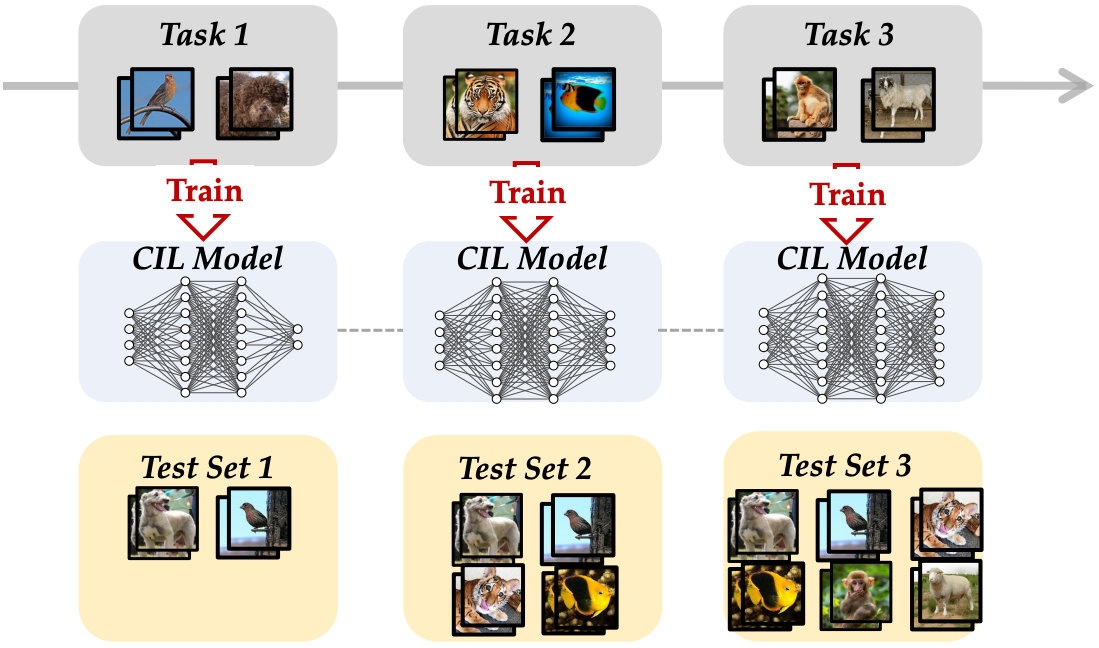
\includegraphics[width=0.9\columnwidth]{images/cil-setup.png}
    \end{center}
    \caption{General CIL setup \cite{zhou2021pycil}.}
    \label{fig:cil-setup}
\end{figure}

During CIL, a stream of class groups $\{\mathcal{Y}_t\}$ and their corresponding training data $\{\mathcal{D}_t\}$ are observed by the model. At step $t$, the incoming dataset $\{\mathcal{D}_t\}$ is of the form $(\textbf{x}_{\textbf{i}}^{\textbf{i}}, y_i^t)$ where $\textbf{x}_{\textbf{i}}^{\textbf{i}}$ is the input image and $y_i^t \in \mathcal{Y}_t$ is the label set $\mathcal{Y}_t$. The label space of the model consists in all the seen categories $\tilde{\mathcal{Y}}_t = \cup_{i=1}^t \mathcal{Y}_i$ and a good model should predict well on all classes $\tilde{\mathcal{Y}}_t$. As described in \autoref{sec:cil-methods}, some CIL algorithms save a part of data at timestamp $t$ as the memory $\mathcal{M}_t$ for future training. The CIL setup is shown in \autoref{fig:cil-setup}.

\subsection{Methods}
\label{sec:cil-methods}


\begin{figure}
    \centerline{
        \begin{forest} for tree={align=center, inner sep=2pt}
        [Class Incremental Learning (CIL)\\methods
        [Replay\\methods
            [Rehearsal
            [
                iCaRL \cite{rebuffi2017icarl}\\
                ER \cite{rolnick2019experience}\\
                SER \cite{isele2018selective}\\
                TEM \cite{chaudhry2019continual}\\
                CoPE \cite{de2021continual}
            ]
            ]
            [Pseudo\\Rehearsal
            [
                DGR \cite{shin2017continual}\\
                PR \cite{atkinson1802pseudo}\\
                CCLUGM \cite{lavda2018continual}\\
                LGM \cite{ramapuram2020lifelong}\\
            ]
            ] 
            [Constrained
            [
                GEM \cite{lopez2017gradient}\\
                A-GEM \cite{chaudhry2018efficient}\\
                GSS \cite{aljundi2019online}\\
            ]
            ] 
        ]
        [Regularization-based\\methods
        [Prior-focused 
            [
                EWC \cite{kirkpatrick2017overcoming}\\
                IMM \cite{lee2017overcoming}\\
                SI \cite{zenke2017continual}\\
                R-EWC \cite{liu2018rotate}\\
                MAS \cite{aljundi2018memory}\\
                Riemannian Walk \cite{chaudhry2018riemannian}\\
            ]
        ]
        [Data-focused 
            [
            LwF \cite{li2017learning}\\
            LFL \cite{jung2016less}\\
            EBLL \cite{rannen2017encoder}\\
            DMC \cite{zhang2020class}\\
            ]
        ]
        ]
        [Parameter\\isolation methods
        [Fixed\\Network
            [
                PackNet \cite{mallya2018packnet}\\
                PathNet \cite{fernando2017pathnet}\\
                Piggybak \cite{mallya2018piggyback}\\
                HAT \cite{serra2018overcoming}\\
            ]
        ]
        [Dynamic\\Network
            [
                PNN \cite{rusu2016progressive}\\
                Expert Gate \cite{aljundi2017expert}\\
                RCL \cite{xu2018reinforced}\\
                DAN \cite{rosenfeld2018incremental}\\
            ]    
        ]]
        ]
        \end{forest}
    }
    \caption{CIL algorithms taxonomy presented in \cite{delange2021continual}.}
    \label{fig:cil-taxonomy}

\end{figure}


     

The problem of CIL has been addressed using different methods, and they can be divided into three main categories and their sub-categories. The taxonomy and the list of algorithms, summarized in the \autoref{fig:cil-taxonomy}, is based on these works \cite{liu2021adaptive, delange2021continual}:

 

\begin{enumerate}
    \item \textbf{Replay methods}: these works stores samples of old classes which are replayed while learning a new task, by doing so it is possible to alleviate forgetting.
    The samples are either reused as model inputs for rehearsal, or to constrain the optimization of loss on the new tasks.

    \begin{enumerate}
        \item \textit{Rehearsal} \cite{rebuffi2017icarl, rolnick2019experience, isele2018selective, chaudhry2019continual, de2021continual}: the model is retrained on a limited subset of stored samples.
        \item \textit{Pseudo Rehearsal} \cite{shin2017continual, atkinson1802pseudo, lavda2018continual, ramapuram2020lifelong}: approximates previous tasks samples using either random input vector or more advanced techniques like generative models. However, the latter one has the drawback of adding complexity to the system pipeline.
        \item \textit{Constrained optimization} \cite{lopez2017gradient, chaudhry2018efficient, aljundi2019online}: updates model's weights for the new task in such a way not to interfere with previous task weights.
    \end{enumerate}
    
    \item \textbf{Regularization-based methods}: these works do not store raw data and reduce the memory requirements. An extra regularization term is introduced in the loss function, in this way it is possible to learn new classes while maintaining the previous knowledge.
    \begin{enumerate}
        \item \textit{Prior-focused methods} \cite{kirkpatrick2017overcoming, lee2017overcoming, zenke2017continual, liu2018rotate, aljundi2018memory, chaudhry2018riemannian}: this approach tries to estimate the importance of the neural network parameters to avoid forgetting as much as possible. Then, when training on new tasks, the optimization process penalizes changes to important weights.
        \item \textit{Data-focused methods} \cite{li2017learning, jung2016less, zhang2020class, rannen2017encoder}: this approach uses knowledge distillation \cite{hinton2015distilling} treating the old model trained on the previous task as the \textit{teacher}, and use it combined with the new data to train the \textit{student} model.
    \end{enumerate}
    \item \textbf{Parameter isolation methods}: this class of methods use different model parameters for each task.
    \begin{enumerate}
        \item \textit{Fixed Network} \cite{mallya2018packnet, mallya2018piggyback, serra2018overcoming, fernando2017pathnet}: the model architecture is kept fixed and the knowledge is updated involving masks for the parameters' weights.
        \item \textit{Dynamic Architectures} \cite{rusu2016progressive, xu2018reinforced, aljundi2017expert, rosenfeld2018incremental}: the model architecture dynamically changes after each incremental task, and the old parameters are freezed to prevent forgetting. Another approach is to dedicate a model to each incremental task.
    \end{enumerate}
\end{enumerate}

Since there are several different algorithms for CIL, the work presented by Zhou et al. in \cite{zhou2021pycil} aims to compare a subset of these algorithms considering the same experimental setup. To this purpose, they publish a repository\footnote{PyCIL GitHub repository: \href{https://github.com/G-U-N/PyCIL}{https://github.com/G-U-N/PyCIL}}
on GitHub where they introduce \textit{PyCIL: A Python Toolbox for Class-Incremental Learning}, which is an implementation of all the following algorithms:

\begin{itemize}
    \item \textbf{Finetune}: the baseline method which updates parameters on new tasks and
    suffers from severe catastrophic forgetting.
    \item \textbf{Replay}: the baseline method which updates parameters on new task with instances
    from the new dataset and exemplar set.
    \item \textbf{EWC} \cite{kirkpatrick2017overcoming}: uses Fisher Information Matrix to weigh the
    importance of each parameter and regularizes important parameters to overcome forgetting.
    \item \textbf{LwF} \cite{li2017learning}: uses knowledge distillation \cite{hinton2015distilling} to
    align the output probability between old and new model.
    \item \textbf{iCaRL} \cite{rebuffi2017icarl}: uses knowledge distillation  \cite{hinton2015distilling}  to
    align the output probability between old and new model. Moreover, it also introduces
    exemplar set for rehearsal and uses nearest center mean classifier.
    \item \textbf{GEM} \cite{lopez2017gradient}: uses exemplars as the regularization of
    gradient updating.
    \item \textbf{BiC} \cite{wu2019large}: trains an extra adaptation layer based on iCaRL, which
    adjusts the logits on new classes.
    \item \textbf{WA} \cite{zhao2020maintaining}: normalizes the classifier weight after each learning session
    based on iCaRL.
    \item \textbf{PODNet} \cite{douillard2020podnet}: introduces a novel distillation loss (Pooled
    Outputs Distillation) constraining the whole convolutional network.
    \item \textbf{DER} \cite{yan2021dynamically}: a two-stage learning approach that utilizes a dynamically
    expandable representation for more effective incremental concept modeling.
    \item \textbf{Coil} \cite{zhou2021co}: builds bi-directional knowledge transfer in the classincremental learning process with optimal transport \cite{villani2009optimal}. It first addresses
    the ability that old model can help learning new classes.
\end{itemize}

The CIL algorithms are tested on two different benchmark datasets, i.e. CIFAR100 and ImageNet100. These datasets are composed of 100 classes and the experiments performed in PyCIL \cite{zhou2021pycil} adopt this CIL setup: 10 classes for the initial stage followed by 9 incremental learning iterations consisting of 10 new classes. Then, the top-1 accuracy is reported for all the incremental stages.
The results are shown in \autoref{fig:cil-comaprison} and the top-1 accuracy at the final stage is reported in \autoref{table:cil-results}.

\begin{figure}%
	\centering
	\subfloat[\centering 10 stage on CIFAR100]{{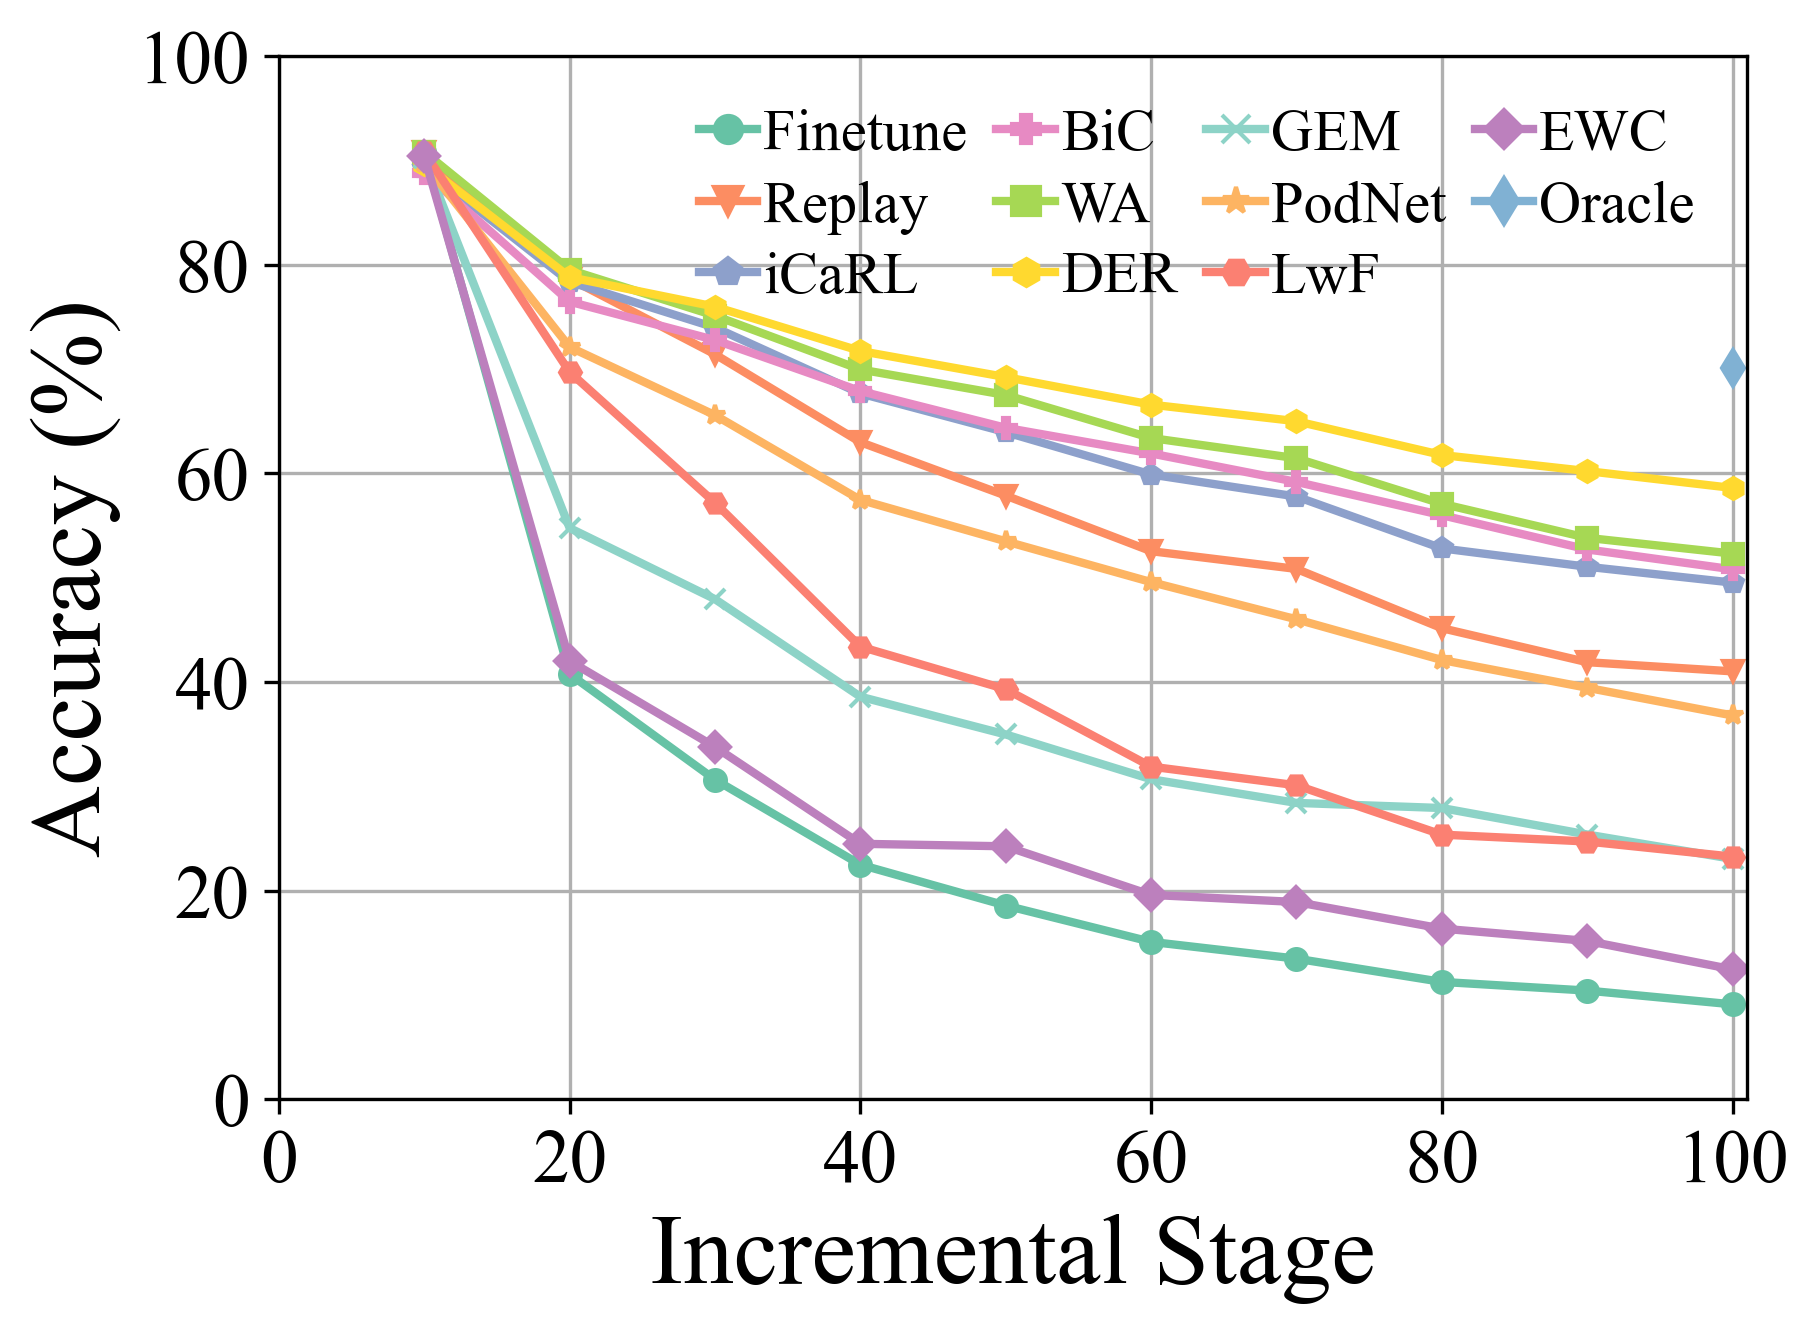
\includegraphics[width=0.45\textwidth]{images/cil-cifar.png} }}%
	\hfill
	\subfloat[\centering 10 stage on ImageNet100]{{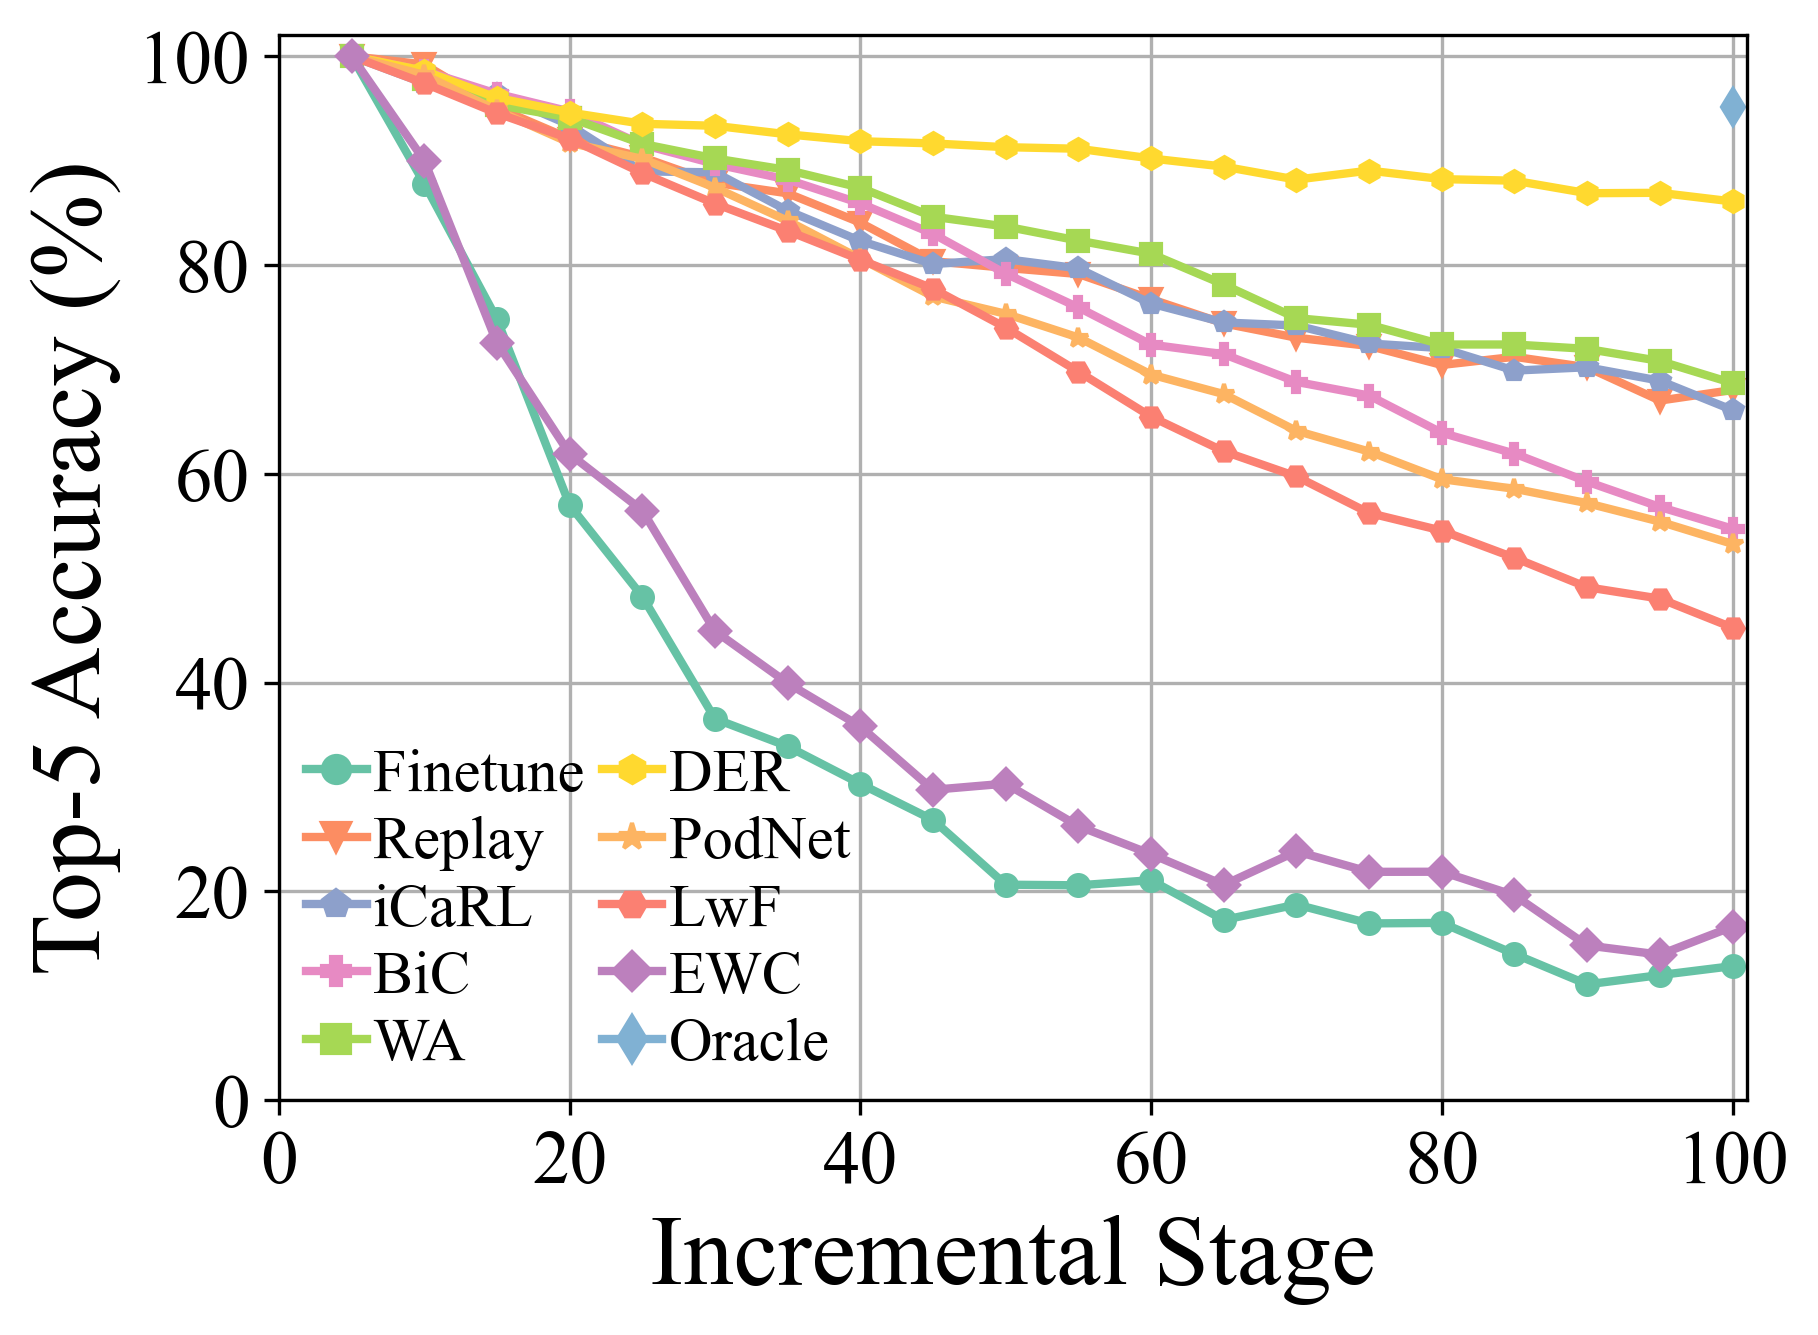
\includegraphics[width=0.45\textwidth]{images/cil-imagenet} }}%
	\caption{Performance comparison of the CIL algorithms during 10 stages on CIFAR100 and ImageNet100 datasets \cite{zhou2021pycil}.}%
	\label{fig:cil-comaprison}%
\end{figure}

\begin{table}
    \centering
    \begin{tabular}{c c} 
     \hline
     \textbf{Method} & \textbf{Top-1 accuracy} \\
     & \textbf{(last stage)}\\
     \hline
     Finetune & 26.25 \\ 
    Replay & 59.31 \\ 
    GEM & 40.18 \\ 
    LwF & 43.56 \\ 
    iCaRL & 64.42 \\ 
    EWC & 29.73 \\ 
    WA & 67.09 \\ 
    PODNet & 55.22 \\ 
    BiC & 65.08 \\ 
    Coil & 65.48 \\ 
    DER & 69.74 \\ 

     \hline
    \end{tabular}
    \caption{Top-1 accuracy of the CIL algorithms at the $10$-th incremental stage using the CIFAR100 dataset \cite{zhou2021pycil}.}
    \label{table:cil-results}
    \end{table}

From the final results reported in PyCIL in \autoref{table:cil-results} it is clear that the best performing algorithm on the considered datasets is DER \cite{yan2021dynamically}. Moreover, even if the authors of PyCIL re-implement the DER algorithm, they point out how the performance obtained from the implementation of PyCIL is very similar to that reported in the original DER paper (69.74 top-1 accuracy in PyCIL vs 69.41 reported by the DER paper).


\subsection{DER: an algorithm for class incremental learning}
DER (dynamically expandable representation) is an algorithm for CIL based on a two-stage learning approach that utilizes a dynamically expandable representation and uses a limited memory for the old classes introduced in each incremental step. The system proposed in this thesis takes advantage of this algorithm for what concerns the incremental learning aspect (see \autoref{sec:method-cil}).


\begin{figure}%
	\centering

    \begin{center}
        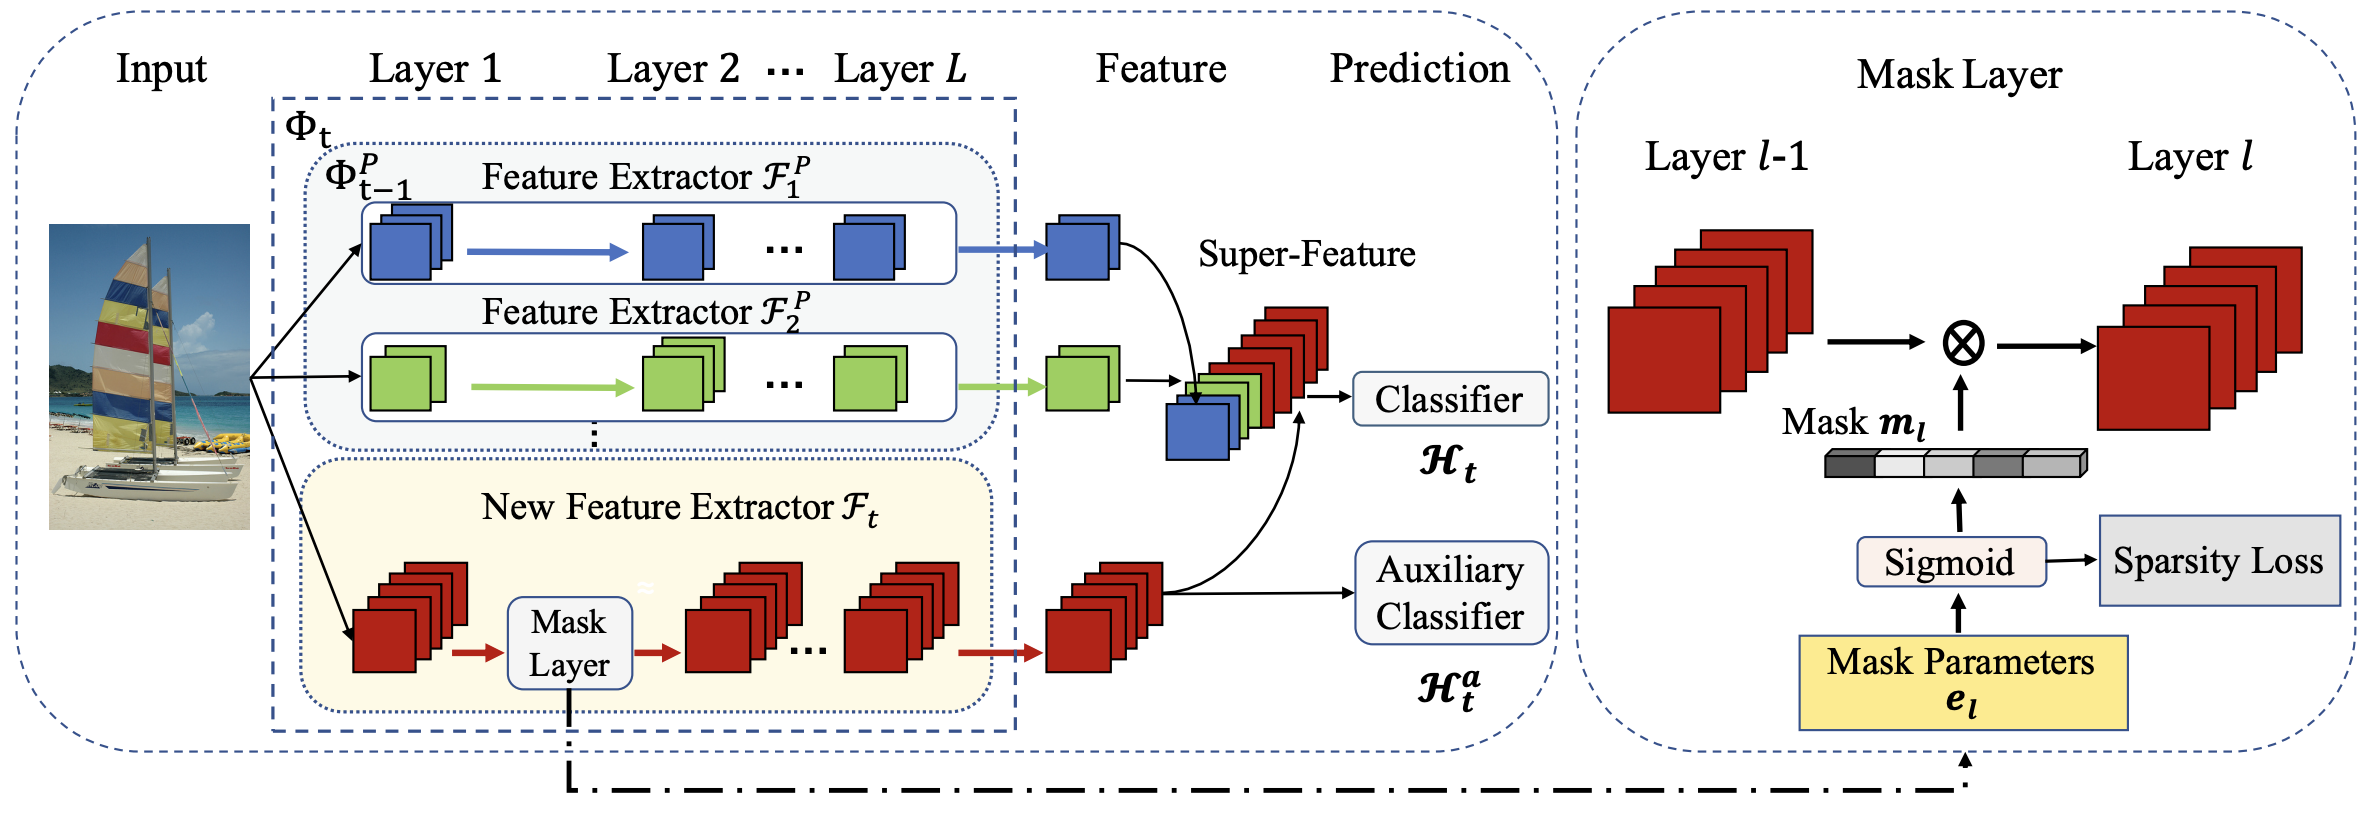
\includegraphics[width=\columnwidth]{images/der-pipeline.png}
    \end{center}

	\caption{Dynamically Expandable Representation Learning method \cite{yan2021dynamically}.}%
	\label{fig:der-pipeline}%
\end{figure}


The DER algorithm described in \cite{yan2021dynamically} can be divided into three stages (see \autoref{fig:der-pipeline}):
\begin{enumerate}
    \item \textbf{Representation Learning Stage}: the architecture of the Convolutional Neural Network (CNN) is dynamically expanded at each new incremental learning iteration.
    \item \textbf{Masking and Pruning}: the CNN introduced in the last incremental learning stage is pruned using a channel-level masked-based method.
    \item \textbf{Classifier Learning Stage}: retrain the classifier with currently available data $\tilde{\mathcal{D}}_t = \mathcal{D}_t \cup \mathcal{M}_t$ at step $t$.
\end{enumerate}

\subsubsection{Expandable Representation Learning}
At step $t$ of the incremental learning, the algorithm defines a super-feature extractor $\Phi_t$ and the classifier $\mathcal{H}_t$. The algorithm expands the neural network architecture at each step by considering the previous super-feature extractor $\Phi_{t-1}$ and a newly created feature extractor $\mathcal{F}_t$. The feature extractor $\mathcal{F}_t$ consists of a CNN, and the classifier $\mathcal{H}_t$ is a Fully Connected (FC) layer after the super-feature extractor $\Phi_t$.

Given an image $\textbf{x} \in \tilde{\mathcal{D}}_t$, the feature $u$ extracted by $\Phi_t$ is the result of the following concatenation:
\begin{equation}
    \textbf{u} = \Phi_t(\textbf{x}) = [\Phi_{t-1}(\textbf{x}), \mathcal{F}_t(x)]
\end{equation}
The feature $\textbf{u}$ is then fed into the classifier $\mathcal{H}_t$, which is defined in such a way that the input and output dimensions for step $t$ match. Then, the prediction is produced as follows:
\begin{equation} \label{eq:classification}
    p_{\mathcal{H}_t}(\textbf{y} | \textbf{x}) = \text{Softmax}(\mathcal{H}_t(\textbf{u}))
\end{equation}
Finally, the actual predicted class is given by:
\begin{equation}
    \hat{y} = \argmax \mathcal{H}_t(\textbf{y} | \textbf{x}), \quad \hat{y} \in \tilde{\mathcal{Y}}_t
\end{equation}
The stability-plasticity tradeoff is taken into account considering these two aspects:
\begin{itemize}
    \item To \textbf{retain old knowledge}, the parameters of $\mathcal{H}_t$ for the old features are inherited from $\mathcal{H}_{t-1}$, and its newly added parameters are randomly initialized.
    \item To \textbf{reduce catastrophic forgetting}, the parameters $\theta_{\Phi_{t-1}}$ and the statistics of Batch Normalization \cite{ioffe2015batch} of the old super-feature extractor $\Phi_{t-1}$ are freezed at step $t$, in this way it is possible to maintain the previously learned knowledge.
\end{itemize}


To force the network to learn new and discriminative features at each incremental step, the authors of the algorithm introduce an auxiliary classifier $\mathcal{H}_t^a$. The label space of $\mathcal{H}_t^a$ is $|\mathcal{Y}_t| + 1$, corresponding to the the set $\mathcal{Y}_t$ of all new categories, and treating all the old concepts as a single category. This is done to encourage the network to learn features that discriminate old and new concepts. The classifier $\mathcal{H}_t^a$ predicts the probability:
\begin{equation} \label{eq:loss-aux}
    p_{\mathcal{H}_t^a}(\textbf{y}|\textbf{x}) = \text{Softmax}(\mathcal{H}_t^a(\mathcal{F}(\textbf{x})))
\end{equation}

\subsubsection{Masking and pruning}
To maintain a compact representation of the model and remove redundancy, the super-feature extractor is pruned after the training of each stage $t$, the method proposed by the authors is adapted from \cite{serra2018overcoming}. This is done using a differentiable channel-level mask-based method to prune filters of the extractor $\mathcal{F}_t$, in which
the masks are learned jointly with the representation. The mask is then binarized after the learning procedure, and the feature extractor $\mathcal{F}_t$ is pruned using the binary mask, producing as output the pruned network $\mathcal{F}_t^{P}$.

Given a new feature extractor $\mathcal{F}_t$, the input feature map of the convolutional layer $l$ for an image $\textbf{x}$ is denoted as $\textbf{f}_l$. The channel mask $\textbf{m}_l \in \mathbb{R}^{c_l}$ controls the size of the layer $l$, where $m_l^i \in [0, 1]$ and $c_l$ is the number of channels of layer $l$. The mask $m_l$ is used to modulate $f_l$ as follows:

\begin{equation}
    \textbf{f}_l \kern 0.05em ' = \textbf{f}_l \odot \textbf{m}_l
\end{equation}
where $\textbf{f}_l \kern 0.05em '$ is the masked feature map and $\odot$ means channel-level multiplication. To make the values of $\textbf{m}_l$ fall into the interval $[0,1]$, the masks is given by:
\begin{equation}
    \textbf{m}_l = \sigma(s \textbf{e}_l)
\end{equation}
where $\textbf{e}_l$ is the learnable mask parameters, $\sigma(\cdot)$ is the sigmoid used as gating function, and $s$ is a scaling factor to control the sharpness of the function.


Using the pruning mechanism, the super-feature $\tilde{\textbf{u}}$ of step $t$ can be rewritten as:
\begin{equation}
    \tilde{\textbf{u}} = \Phi_t^P(\textbf{x}) = [\mathcal{F}_1^P, \mathcal{F}_2^P,\, ..., \phi(\textbf{x})]
\end{equation}

During the training $\phi_t(\textbf{x})$ corresponds to $\mathcal{F}_t(\textbf{x})$ with the soft mask. At inference time, thanks to the scaling factor $s$, the masks associated to the filters of the convolutional layers are pruned assigning a large value to $s$. In this way the it is possible to obtain $\mathcal{F}_t^P = \phi_t(\textbf{x})$.

The parameters $\textbf{e}_l$ which define the masks are learned during training. During an epoch, a linear annealing schedule is applied for $s$ as follows:
\begin{equation}
    s = \frac{1}{s_{max}} + (s_{max}- \frac{1}{s_{max}}) \frac{b-1}{B-1}
\end{equation}
where $b$ is the batch index, $B$ is the number of batches in one epoch, and $s_{max} \gg 1$ is a hyperparameter.

In this way, at the start of the training epoch, $s$ has a small value. Thus, given that $\textbf{m}_l=\sigma(s \textbf{e}_l)$, the gating mechanism leads to values close to $0.5$, regardless of the $\textbf{e}_l$ vector. Then the mask is progressively binarized with the increasing of the batch index $b$ within a epoch.

As described in \cite{serra2018overcoming}, to solve the problem of the unstable gradient of $\textbf{e}_l$ due to the $s$ schedule, the gradient $\textbf{g}_{\textbf{e}_l}$ with respect to $\textbf{e}_l$ is compensated as follows:
\begin{equation}
    \textbf{g}_{\textbf{e}_l} ' = \frac{\sigma(\textbf{e}_l)[1-\sigma(\textbf{e}_l)]}{s\sigma(s\textbf{e}_l)[1-\sigma(s\textbf{e}_l)]}\textbf{g}_{\textbf{e}_l}
\end{equation}
where $\textbf{g}_{\textbf{e}_l} '$ is the compensated gradient.


\subsubsection{Classifier Learning}
After the representation learning stage, the classifier head is re-trained to reduce the bias in the classifier weight introduced by the imbalanced training set $\tilde{\mathcal{D}}_t$, this is due to the difference in sample size between the old classes in the memory $\mathcal{M}_t$ and the currently available data $\mathcal{D}_t$. To this purpose, the classifier weight are randomly initialized and the classifier is trained on a class-balanced sample of $\tilde{\mathcal{D}}_t$ using the cross-entropy loss with a temperature $\delta$ in the Softmax presented in \cite{zhao2020maintaining}. 

\subsubsection{Loss function}
The loss function used to change the parameters of the model is defined by three components:

\begin{enumerate}
    \item \textbf{Classifier Loss}: the first loss component is responsible for the correct classification of all the images. Hence, based on the \autoref{eq:classification}, given an image and its corresponding label $(\textbf{x}_i, y_i)\in \tilde{\mathcal{D}}$, the loss function penalizes wrong class prediction as follows:
    \begin{equation} \label{eq:loss1}
        \mathcal{L}_{\mathcal{H}_t} = - \frac{1}{|\tilde{\mathcal{D}}_t|}
            \sum_{i=1}^{|\tilde{\mathcal{D}}_t|}log(p_{\mathcal{H}_t}(y=y_i | \textbf{x}_i))
    \end{equation}
    \item \textbf{Auxiliary Loss}: the second loss component is relative to the auxiliary classifier $\mathcal{H}_t^a$. Consistently with \autoref{eq:loss-aux}, given an image $\textbf{x}_i$ and the associated label $y_i \in \mathcal{Y}_i \cup \{"old"\}$, the auxiliary loss component is defined as follows:
    \begin{equation} \label{eq:loss2}
        \mathcal{L}_{\mathcal{H}_t^a} = - \frac{1}{|\tilde{\mathcal{D}}_t|}
            \sum_{i=1}^{|\tilde{\mathcal{D}}_t|}log(p_{\mathcal{H}_t}(y=y_i | \textbf{x}_i))
    \end{equation}
    \item \textbf{Sparsity Loss}: the third loss component encourage the model to maximally reduce the number of parameters with a minimal performance drop. To this reason the sparsity loss considers the ratio of used weights in all available weights:
    \begin{equation} \label{eq:loss3}
        \mathcal{L}_S = \frac{\sum_{l=1}^L K_l \| \textbf{m}_{l-1} \|_1  \| \textbf{m}_{l} \|_1 }{\sum_{l=1}^L K_l c_{l-1} c_{l}}
    \end{equation}
    where $L$ is the number of layers and $K_l$ is the kernel size of convolutional layer $l$.
\end{enumerate}

The final loss function is given by the weighted average of \autoref{eq:loss1}, \autoref{eq:loss2} and \autoref{eq:loss3}:
\begin{equation}
    \mathcal{L}_{DER} = \mathcal{L}_{\mathcal{H}_t} + \lambda_a \mathcal{L}_{\mathcal{H}_t^a} + \lambda_s \mathcal{L}_{S}
\end{equation}
where $\lambda_a$ and $\lambda_s$ are the hyper-parameter to control the effect of the auxiliary classifier and the pruning aspect.

\section{Weight aligning}
Weight aligning (WA) proposed in \cite{zhao2020maintaining} is a method to alleviate catastrophic forgetting in DNN. In their work the authors show how a model trained for a CIL task tends
to classify objects into new classes, treating old classes unfairly. This is due to the weights
in the trained model's FC layer which are heavily biased. WA aims to correct bias in the FC layer.

\subsubsection{Biased Weights in the FC Layer}
\label{sec:wa-biased}
At the $t$-th incremental learning step, the model is given by:
\begin{equation}
    o(\textbf{x}) = \textbf{W}^T \Phi(\textbf{x})
\end{equation}
where:
\begin{itemize}
    \item $\Phi(\textbf{x})$ is the feature extractor which output a $d$-dimensional feature vector.
    \item $o(\textbf{x})$ is the ($C_{old}^t + C^t$)-dimensional vector of the logits produced in output by the model. $C_{old}^t$ and $C^t$ represent respectively the number of old and new classes at the $t$-th incremental stage. 
    \item $W \in \mathbb{R}^{d \times (C_{old}^t + C^t)}$ represents the parameters of the FC layer. $W$ can be espressed as $W = {w_c, \, 1 \leq c \leq C_{old}^b + C^b}$, where $w_c$ is a $d$-dimensional weight vector for the $c^{th}$ class.
\end{itemize}
The output logits for the $c^{th}$ class is calculated as:
\begin{equation}
    o_c(\textbf{x}) = \textbf{w}_c^T \Phi (\textbf{x})
\end{equation}
The motivation behind WA is the observation that the norms of weight vectors for new classes are larger, thus leading the output logits for new classes to be larger in general. As a result, the biased FC layer in the model tends to predict an input image as belonging to a new class. This analysis emerges from the experiments performed in \cite{zhao2020maintaining} shown in \autoref{fig:wa-biased}.
\begin{figure}%
    \hspace*{-1.25 cm}
	\subfloat[$C^0=20,C_{old}^0=0$]{{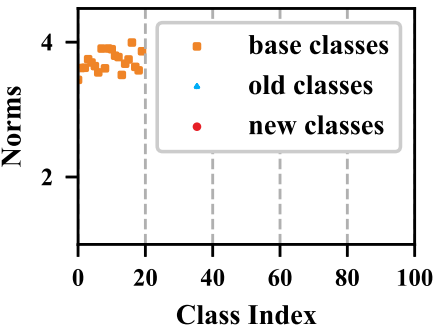
\includegraphics[width=0.22\textwidth]{images/wa-biased_1.png} }}
	\subfloat[$C^1=20,C_{old}^1=20$]{{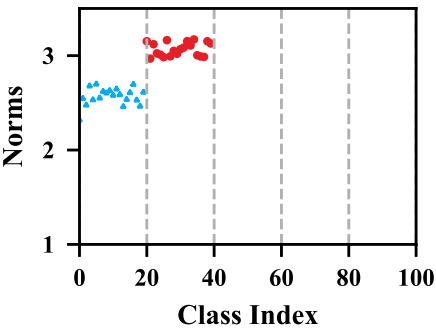
\includegraphics[width=0.22\textwidth]{images/wa-biased_2.png} }}
	\subfloat[$C^2=20,C_{old}^2=40$]{{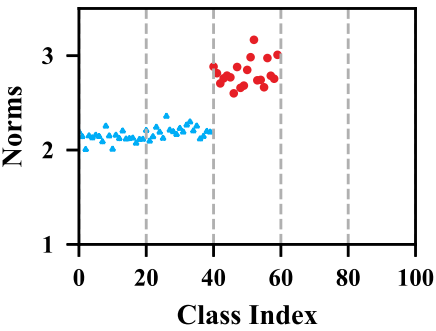
\includegraphics[width=0.22\textwidth]{images/wa-biased_3.png} }}
	\subfloat[$C^3=20,C_{old}^3=60$]{{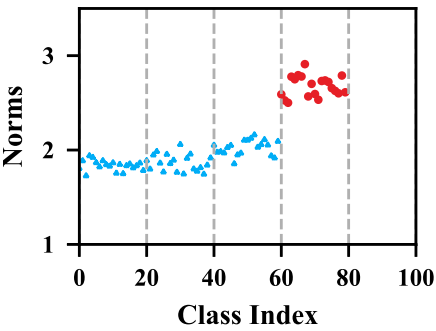
\includegraphics[width=0.22\textwidth]{images/wa-biased_4.png} }}
	\subfloat[$C^4=20,C_{old}^4=80$]{{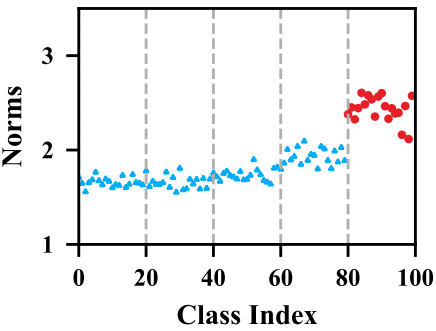
\includegraphics[width=0.22\textwidth]{images/wa-biased_5.png} }}
	\caption{Norm of the weight vectors $\{\textbf{w}_c\}$ after each incremental step. (a) Represents the initial step; (b), (c), (d), (e) are the $1^{st}$, $2^{nd}$, $3^{rd}$ and $4^{th}$ incremental step. The figure show the difference in the norms of the weight between the old and new classes \cite{zhao2020maintaining}.}%
	\label{fig:wa-biased}
\end{figure}

\subsubsection{Correct the biased weights in the FC Layer}
The bias in the weights of the FC layer described in \autoref{sec:wa-biased} is corrected using the WA tec.  The FC layer can be rewritten as $\textbf{W} = (\textbf{W}_{old}, \textbf{W}_{new})$, where 
$$\textbf{W}_{old} = (\textbf{w}_1, \textbf{w}_2, \, ..., \textbf{w}_{C_{old}^t}) \in \mathbb{R}^{d \times C_{old}^t},$$
$$\textbf{W}_{new} = (\textbf{w}_{C_{old}^t + 1}, \, ..., \textbf{w}_{C_{old}^t + C^t}) \in \mathbb{R}^{d \times C^t}.$$
The norms of the weight vectors of old and new classes can be denoted by:
$$\textbf{Norm}_{old} = (\| \textbf{w}_1 \|,  \, ..., \| \textbf{w}_{C_{old}^t \|}),$$
$$\textbf{Norm}_{new} = (\| \textbf{w}_{C_{old}^t + 1} \|, \, ..., \| \textbf{w}_{C_{old}^t + C^t} \|).$$
Then, the weights for new classes is normalized as follows:
\begin{equation}
    \hat{\textbf{W}}_{new} = \gamma \cdot \textbf{W}_{new}
\end{equation}
where
\begin{equation}
    \gamma = \frac{Mean(\textbf{Norm}_{old} )}{Mean(\textbf{Norm}_{new})}
\end{equation}
$Mean(\cdot)$ returns the mean value of elements in the vector.

This correction on the FC layer directly affects the output logits produced by the model. In fact, the output logits of the model before WA can be expressed as:
\begin{equation}
    \begin{split}
        \textbf{o}(\textbf{x}) = &\; (\textbf{o}_{old}(\textbf{x}), \textbf{o}_{new}(\textbf{x}))^T \\
        = &\; (\textbf{W}_{old}^T \Phi(\textbf{x}), \textbf{W}_{new}^T \Phi(\textbf{x}) )^T
    \end{split}
\end{equation}
after applying WA on the FC, the corrected output logits are given by:
\begin{equation}
    \begin{split}
        \textbf{o}_{corrected}(\textbf{x})
        = &\; (\textbf{W}_{old}^T \Phi(\textbf{x}), \hat{\textbf{W}}_{new}^T \Phi(\textbf{x}))^T \\
        = &\; (\textbf{W}_{old}^T \Phi(\textbf{x}), \gamma \cdot \textbf{W}_{new}^T \Phi(\textbf{x}))^T \\
        = &\; (\textbf{o}_{old}(\textbf{x}), \gamma \cdot \textbf{o}_{new}(\textbf{x}))^T
    \end{split}
\end{equation}

The final effect of aligning the weights is to rescale the output logits of new classes, thus leading to a fair classification between old and new classes.